% Created by tikzDevice version 0.7.0 on 2014-07-26 02:56:00
% !TEX encoding = UTF-8 Unicode
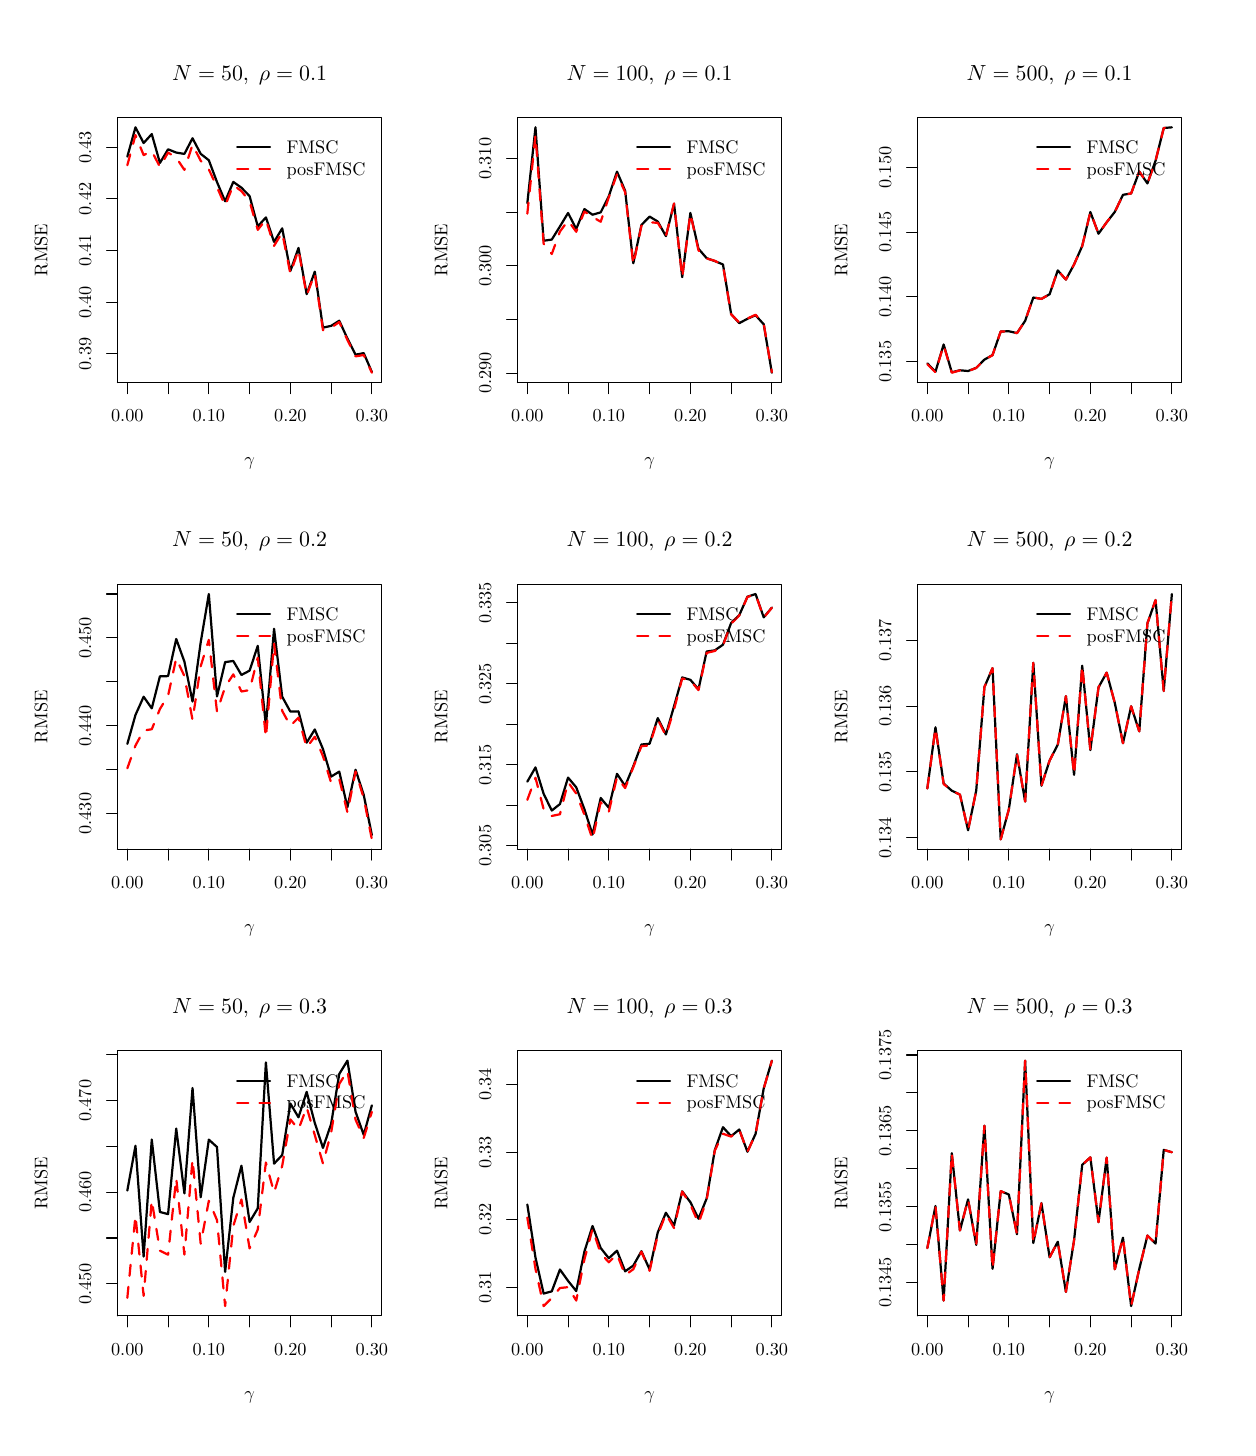
\begin{tikzpicture}[x=1pt,y=1pt]
\definecolor[named]{fillColor}{rgb}{1.00,1.00,1.00}
\path[use as bounding box,fill=fillColor,fill opacity=0.00] (0,0) rectangle (433.62,505.89);
\begin{scope}
\path[clip] ( 32.47,377.65) rectangle (127.91,473.42);
\definecolor[named]{drawColor}{rgb}{0.00,0.00,0.00}

\path[draw=drawColor,line width= 0.8pt,line join=round,line cap=round] ( 36.01,459.27) --
	( 38.95,469.87) --
	( 41.90,464.20) --
	( 44.84,467.44) --
	( 47.79,457.01) --
	( 50.73,461.94) --
	( 53.68,460.75) --
	( 56.63,460.27) --
	( 59.57,465.93) --
	( 62.52,460.29) --
	( 65.46,457.98) --
	( 68.41,450.10) --
	( 71.35,443.15) --
	( 74.30,450.15) --
	( 77.24,448.06) --
	( 80.19,445.03) --
	( 83.14,434.09) --
	( 86.08,437.32) --
	( 89.03,428.46) --
	( 91.97,433.38) --
	( 94.92,417.95) --
	( 97.86,426.29) --
	(100.81,409.59) --
	(103.75,417.72) --
	(106.70,397.48) --
	(109.65,398.14) --
	(112.59,399.99) --
	(115.54,393.54) --
	(118.48,387.71) --
	(121.43,388.29) --
	(124.37,381.47);
\end{scope}
\begin{scope}
\path[clip] (  0.00,  0.00) rectangle (433.62,505.89);
\definecolor[named]{drawColor}{rgb}{0.00,0.00,0.00}

\path[draw=drawColor,line width= 0.4pt,line join=round,line cap=round] ( 36.01,377.65) -- (124.37,377.65);

\path[draw=drawColor,line width= 0.4pt,line join=round,line cap=round] ( 36.01,377.65) -- ( 36.01,373.69);

\path[draw=drawColor,line width= 0.4pt,line join=round,line cap=round] ( 50.73,377.65) -- ( 50.73,373.69);

\path[draw=drawColor,line width= 0.4pt,line join=round,line cap=round] ( 65.46,377.65) -- ( 65.46,373.69);

\path[draw=drawColor,line width= 0.4pt,line join=round,line cap=round] ( 80.19,377.65) -- ( 80.19,373.69);

\path[draw=drawColor,line width= 0.4pt,line join=round,line cap=round] ( 94.92,377.65) -- ( 94.92,373.69);

\path[draw=drawColor,line width= 0.4pt,line join=round,line cap=round] (109.65,377.65) -- (109.65,373.69);

\path[draw=drawColor,line width= 0.4pt,line join=round,line cap=round] (124.37,377.65) -- (124.37,373.69);

\node[text=drawColor,anchor=base,inner sep=0pt, outer sep=0pt, scale=  0.66] at ( 36.01,363.40) {0.00};

\node[text=drawColor,anchor=base,inner sep=0pt, outer sep=0pt, scale=  0.66] at ( 65.46,363.40) {0.10};

\node[text=drawColor,anchor=base,inner sep=0pt, outer sep=0pt, scale=  0.66] at ( 94.92,363.40) {0.20};

\node[text=drawColor,anchor=base,inner sep=0pt, outer sep=0pt, scale=  0.66] at (124.37,363.40) {0.30};

\path[draw=drawColor,line width= 0.4pt,line join=round,line cap=round] ( 32.47,388.00) -- ( 32.47,462.68);

\path[draw=drawColor,line width= 0.4pt,line join=round,line cap=round] ( 32.47,388.00) -- ( 28.51,388.00);

\path[draw=drawColor,line width= 0.4pt,line join=round,line cap=round] ( 32.47,406.67) -- ( 28.51,406.67);

\path[draw=drawColor,line width= 0.4pt,line join=round,line cap=round] ( 32.47,425.34) -- ( 28.51,425.34);

\path[draw=drawColor,line width= 0.4pt,line join=round,line cap=round] ( 32.47,444.01) -- ( 28.51,444.01);

\path[draw=drawColor,line width= 0.4pt,line join=round,line cap=round] ( 32.47,462.68) -- ( 28.51,462.68);

\node[text=drawColor,rotate= 90.00,anchor=base,inner sep=0pt, outer sep=0pt, scale=  0.66] at ( 22.97,388.00) {0.39};

\node[text=drawColor,rotate= 90.00,anchor=base,inner sep=0pt, outer sep=0pt, scale=  0.66] at ( 22.97,406.67) {0.40};

\node[text=drawColor,rotate= 90.00,anchor=base,inner sep=0pt, outer sep=0pt, scale=  0.66] at ( 22.97,425.34) {0.41};

\node[text=drawColor,rotate= 90.00,anchor=base,inner sep=0pt, outer sep=0pt, scale=  0.66] at ( 22.97,444.01) {0.42};

\node[text=drawColor,rotate= 90.00,anchor=base,inner sep=0pt, outer sep=0pt, scale=  0.66] at ( 22.97,462.68) {0.43};

\path[draw=drawColor,line width= 0.4pt,line join=round,line cap=round] ( 32.47,377.65) --
	(127.91,377.65) --
	(127.91,473.42) --
	( 32.47,473.42) --
	( 32.47,377.65);
\end{scope}
\begin{scope}
\path[clip] (  0.00,337.26) rectangle (144.54,505.89);
\definecolor[named]{drawColor}{rgb}{0.00,0.00,0.00}

\node[text=drawColor,anchor=base,inner sep=0pt, outer sep=0pt, scale=  0.79] at ( 80.19,486.92) {\bfseries $N=50, \;\rho=0.1$};

\node[text=drawColor,anchor=base,inner sep=0pt, outer sep=0pt, scale=  0.66] at ( 80.19,347.56) {$\gamma$};

\node[text=drawColor,rotate= 90.00,anchor=base,inner sep=0pt, outer sep=0pt, scale=  0.66] at (  7.13,425.54) {RMSE};
\end{scope}
\begin{scope}
\path[clip] ( 32.47,377.65) rectangle (127.91,473.42);
\definecolor[named]{drawColor}{rgb}{1.00,0.00,0.00}

\path[draw=drawColor,line width= 0.8pt,dash pattern=on 4pt off 4pt ,line join=round,line cap=round] ( 36.01,456.18) --
	( 38.95,467.06) --
	( 41.90,459.85) --
	( 44.84,461.28) --
	( 47.79,455.56) --
	( 50.73,460.76) --
	( 53.68,458.93) --
	( 56.63,454.50) --
	( 59.57,463.59) --
	( 62.52,457.79) --
	( 65.46,454.67) --
	( 68.41,448.28) --
	( 71.35,441.53) --
	( 74.30,448.99) --
	( 77.24,446.83) --
	( 80.19,443.12) --
	( 83.14,432.82) --
	( 86.08,436.55) --
	( 89.03,427.06) --
	( 91.97,431.85) --
	( 94.92,416.97) --
	( 97.86,425.66) --
	(100.81,409.19) --
	(103.75,417.02) --
	(106.70,396.60) --
	(109.65,397.50) --
	(112.59,399.52) --
	(115.54,393.04) --
	(118.48,387.10) --
	(121.43,387.61) --
	(124.37,381.20);
\definecolor[named]{drawColor}{rgb}{0.00,0.00,0.00}

\path[draw=drawColor,line width= 0.8pt,line join=round,line cap=round] ( 75.72,462.63) -- ( 87.60,462.63);
\definecolor[named]{drawColor}{rgb}{1.00,0.00,0.00}

\path[draw=drawColor,line width= 0.8pt,dash pattern=on 4pt off 4pt ,line join=round,line cap=round] ( 75.72,454.71) -- ( 87.60,454.71);
\definecolor[named]{drawColor}{rgb}{0.00,0.00,0.00}

\node[text=drawColor,anchor=base west,inner sep=0pt, outer sep=0pt, scale=  0.66] at ( 93.54,460.35) {FMSC};

\node[text=drawColor,anchor=base west,inner sep=0pt, outer sep=0pt, scale=  0.66] at ( 93.54,452.43) {posFMSC};
\end{scope}
\begin{scope}
\path[clip] (177.01,377.65) rectangle (272.45,473.42);
\definecolor[named]{drawColor}{rgb}{0.00,0.00,0.00}

\path[draw=drawColor,line width= 0.8pt,line join=round,line cap=round] (180.55,442.46) --
	(183.49,469.87) --
	(186.44,428.89) --
	(189.38,429.31) --
	(192.33,434.06) --
	(195.27,438.93) --
	(198.22,433.14) --
	(201.17,440.34) --
	(204.11,438.30) --
	(207.06,439.15) --
	(210.00,445.04) --
	(212.95,453.86) --
	(215.89,446.96) --
	(218.84,420.75) --
	(221.78,434.60) --
	(224.73,437.62) --
	(227.68,435.83) --
	(230.62,430.56) --
	(233.57,442.29) --
	(236.51,415.74) --
	(239.46,438.94) --
	(242.40,425.98) --
	(245.35,422.59) --
	(248.29,421.55) --
	(251.24,420.32) --
	(254.19,402.42) --
	(257.13,399.11) --
	(260.08,400.69) --
	(263.02,401.97) --
	(265.97,398.70) --
	(268.91,381.20);
\end{scope}
\begin{scope}
\path[clip] (  0.00,  0.00) rectangle (433.62,505.89);
\definecolor[named]{drawColor}{rgb}{0.00,0.00,0.00}

\path[draw=drawColor,line width= 0.4pt,line join=round,line cap=round] (180.55,377.65) -- (268.91,377.65);

\path[draw=drawColor,line width= 0.4pt,line join=round,line cap=round] (180.55,377.65) -- (180.55,373.69);

\path[draw=drawColor,line width= 0.4pt,line join=round,line cap=round] (195.27,377.65) -- (195.27,373.69);

\path[draw=drawColor,line width= 0.4pt,line join=round,line cap=round] (210.00,377.65) -- (210.00,373.69);

\path[draw=drawColor,line width= 0.4pt,line join=round,line cap=round] (224.73,377.65) -- (224.73,373.69);

\path[draw=drawColor,line width= 0.4pt,line join=round,line cap=round] (239.46,377.65) -- (239.46,373.69);

\path[draw=drawColor,line width= 0.4pt,line join=round,line cap=round] (254.19,377.65) -- (254.19,373.69);

\path[draw=drawColor,line width= 0.4pt,line join=round,line cap=round] (268.91,377.65) -- (268.91,373.69);

\node[text=drawColor,anchor=base,inner sep=0pt, outer sep=0pt, scale=  0.66] at (180.55,363.40) {0.00};

\node[text=drawColor,anchor=base,inner sep=0pt, outer sep=0pt, scale=  0.66] at (210.00,363.40) {0.10};

\node[text=drawColor,anchor=base,inner sep=0pt, outer sep=0pt, scale=  0.66] at (239.46,363.40) {0.20};

\node[text=drawColor,anchor=base,inner sep=0pt, outer sep=0pt, scale=  0.66] at (268.91,363.40) {0.30};

\path[draw=drawColor,line width= 0.4pt,line join=round,line cap=round] (177.01,381.05) -- (177.01,458.57);

\path[draw=drawColor,line width= 0.4pt,line join=round,line cap=round] (177.01,381.05) -- (173.05,381.05);

\path[draw=drawColor,line width= 0.4pt,line join=round,line cap=round] (177.01,400.43) -- (173.05,400.43);

\path[draw=drawColor,line width= 0.4pt,line join=round,line cap=round] (177.01,419.81) -- (173.05,419.81);

\path[draw=drawColor,line width= 0.4pt,line join=round,line cap=round] (177.01,439.19) -- (173.05,439.19);

\path[draw=drawColor,line width= 0.4pt,line join=round,line cap=round] (177.01,458.57) -- (173.05,458.57);

\node[text=drawColor,rotate= 90.00,anchor=base,inner sep=0pt, outer sep=0pt, scale=  0.66] at (167.51,381.05) {0.290};

\node[text=drawColor,rotate= 90.00,anchor=base,inner sep=0pt, outer sep=0pt, scale=  0.66] at (167.51,419.81) {0.300};

\node[text=drawColor,rotate= 90.00,anchor=base,inner sep=0pt, outer sep=0pt, scale=  0.66] at (167.51,458.57) {0.310};

\path[draw=drawColor,line width= 0.4pt,line join=round,line cap=round] (177.01,377.65) --
	(272.45,377.65) --
	(272.45,473.42) --
	(177.01,473.42) --
	(177.01,377.65);
\end{scope}
\begin{scope}
\path[clip] (144.54,337.26) rectangle (289.08,505.89);
\definecolor[named]{drawColor}{rgb}{0.00,0.00,0.00}

\node[text=drawColor,anchor=base,inner sep=0pt, outer sep=0pt, scale=  0.79] at (224.73,486.92) {\bfseries $N=100, \;\rho=0.1$};

\node[text=drawColor,anchor=base,inner sep=0pt, outer sep=0pt, scale=  0.66] at (224.73,347.56) {$\gamma$};

\node[text=drawColor,rotate= 90.00,anchor=base,inner sep=0pt, outer sep=0pt, scale=  0.66] at (151.67,425.54) {RMSE};
\end{scope}
\begin{scope}
\path[clip] (177.01,377.65) rectangle (272.45,473.42);
\definecolor[named]{drawColor}{rgb}{1.00,0.00,0.00}

\path[draw=drawColor,line width= 0.8pt,dash pattern=on 4pt off 4pt ,line join=round,line cap=round] (180.55,438.68) --
	(183.49,466.99) --
	(186.44,427.83) --
	(189.38,424.10) --
	(192.33,432.21) --
	(195.27,436.17) --
	(198.22,432.14) --
	(201.17,439.45) --
	(204.11,437.50) --
	(207.06,435.75) --
	(210.00,444.63) --
	(212.95,452.94) --
	(215.89,446.45) --
	(218.84,420.26) --
	(221.78,434.26) --
	(224.73,435.53) --
	(227.68,435.37) --
	(230.62,430.60) --
	(233.57,442.36) --
	(236.51,415.60) --
	(239.46,438.74) --
	(242.40,425.39) --
	(245.35,422.49) --
	(248.29,421.64) --
	(251.24,420.05) --
	(254.19,402.29) --
	(257.13,399.33) --
	(260.08,400.78) --
	(263.02,402.15) --
	(265.97,398.93) --
	(268.91,381.38);
\definecolor[named]{drawColor}{rgb}{0.00,0.00,0.00}

\path[draw=drawColor,line width= 0.8pt,line join=round,line cap=round] (220.26,462.63) -- (232.14,462.63);
\definecolor[named]{drawColor}{rgb}{1.00,0.00,0.00}

\path[draw=drawColor,line width= 0.8pt,dash pattern=on 4pt off 4pt ,line join=round,line cap=round] (220.26,454.71) -- (232.14,454.71);
\definecolor[named]{drawColor}{rgb}{0.00,0.00,0.00}

\node[text=drawColor,anchor=base west,inner sep=0pt, outer sep=0pt, scale=  0.66] at (238.08,460.35) {FMSC};

\node[text=drawColor,anchor=base west,inner sep=0pt, outer sep=0pt, scale=  0.66] at (238.08,452.43) {posFMSC};
\end{scope}
\begin{scope}
\path[clip] (321.55,377.65) rectangle (416.99,473.42);
\definecolor[named]{drawColor}{rgb}{0.00,0.00,0.00}

\path[draw=drawColor,line width= 0.8pt,line join=round,line cap=round] (325.09,384.58) --
	(328.03,381.58) --
	(330.98,391.41) --
	(333.92,381.37) --
	(336.87,382.08) --
	(339.81,381.82) --
	(342.76,382.96) --
	(345.71,385.93) --
	(348.65,387.59) --
	(351.60,396.10) --
	(354.54,396.18) --
	(357.49,395.52) --
	(360.43,399.95) --
	(363.38,408.38) --
	(366.32,407.89) --
	(369.27,409.57) --
	(372.22,418.17) --
	(375.16,414.86) --
	(378.11,420.33) --
	(381.05,426.97) --
	(384.00,439.27) --
	(386.94,431.43) --
	(389.89,435.56) --
	(392.83,439.31) --
	(395.78,445.48) --
	(398.73,445.98) --
	(401.67,453.90) --
	(404.62,449.60) --
	(407.56,457.83) --
	(410.51,469.63) --
	(413.45,469.87);
\end{scope}
\begin{scope}
\path[clip] (  0.00,  0.00) rectangle (433.62,505.89);
\definecolor[named]{drawColor}{rgb}{0.00,0.00,0.00}

\path[draw=drawColor,line width= 0.4pt,line join=round,line cap=round] (325.09,377.65) -- (413.45,377.65);

\path[draw=drawColor,line width= 0.4pt,line join=round,line cap=round] (325.09,377.65) -- (325.09,373.69);

\path[draw=drawColor,line width= 0.4pt,line join=round,line cap=round] (339.81,377.65) -- (339.81,373.69);

\path[draw=drawColor,line width= 0.4pt,line join=round,line cap=round] (354.54,377.65) -- (354.54,373.69);

\path[draw=drawColor,line width= 0.4pt,line join=round,line cap=round] (369.27,377.65) -- (369.27,373.69);

\path[draw=drawColor,line width= 0.4pt,line join=round,line cap=round] (384.00,377.65) -- (384.00,373.69);

\path[draw=drawColor,line width= 0.4pt,line join=round,line cap=round] (398.73,377.65) -- (398.73,373.69);

\path[draw=drawColor,line width= 0.4pt,line join=round,line cap=round] (413.45,377.65) -- (413.45,373.69);

\node[text=drawColor,anchor=base,inner sep=0pt, outer sep=0pt, scale=  0.66] at (325.09,363.40) {0.00};

\node[text=drawColor,anchor=base,inner sep=0pt, outer sep=0pt, scale=  0.66] at (354.54,363.40) {0.10};

\node[text=drawColor,anchor=base,inner sep=0pt, outer sep=0pt, scale=  0.66] at (384.00,363.40) {0.20};

\node[text=drawColor,anchor=base,inner sep=0pt, outer sep=0pt, scale=  0.66] at (413.45,363.40) {0.30};

\path[draw=drawColor,line width= 0.4pt,line join=round,line cap=round] (321.55,385.24) -- (321.55,455.38);

\path[draw=drawColor,line width= 0.4pt,line join=round,line cap=round] (321.55,385.24) -- (317.59,385.24);

\path[draw=drawColor,line width= 0.4pt,line join=round,line cap=round] (321.55,408.62) -- (317.59,408.62);

\path[draw=drawColor,line width= 0.4pt,line join=round,line cap=round] (321.55,432.00) -- (317.59,432.00);

\path[draw=drawColor,line width= 0.4pt,line join=round,line cap=round] (321.55,455.38) -- (317.59,455.38);

\node[text=drawColor,rotate= 90.00,anchor=base,inner sep=0pt, outer sep=0pt, scale=  0.66] at (312.05,385.24) {0.135};

\node[text=drawColor,rotate= 90.00,anchor=base,inner sep=0pt, outer sep=0pt, scale=  0.66] at (312.05,408.62) {0.140};

\node[text=drawColor,rotate= 90.00,anchor=base,inner sep=0pt, outer sep=0pt, scale=  0.66] at (312.05,432.00) {0.145};

\node[text=drawColor,rotate= 90.00,anchor=base,inner sep=0pt, outer sep=0pt, scale=  0.66] at (312.05,455.38) {0.150};

\path[draw=drawColor,line width= 0.4pt,line join=round,line cap=round] (321.55,377.65) --
	(416.99,377.65) --
	(416.99,473.42) --
	(321.55,473.42) --
	(321.55,377.65);
\end{scope}
\begin{scope}
\path[clip] (289.08,337.26) rectangle (433.62,505.89);
\definecolor[named]{drawColor}{rgb}{0.00,0.00,0.00}

\node[text=drawColor,anchor=base,inner sep=0pt, outer sep=0pt, scale=  0.79] at (369.27,486.92) {\bfseries $N=500, \;\rho=0.1$};

\node[text=drawColor,anchor=base,inner sep=0pt, outer sep=0pt, scale=  0.66] at (369.27,347.56) {$\gamma$};

\node[text=drawColor,rotate= 90.00,anchor=base,inner sep=0pt, outer sep=0pt, scale=  0.66] at (296.21,425.53) {RMSE};
\end{scope}
\begin{scope}
\path[clip] (321.55,377.65) rectangle (416.99,473.42);
\definecolor[named]{drawColor}{rgb}{1.00,0.00,0.00}

\path[draw=drawColor,line width= 0.8pt,dash pattern=on 4pt off 4pt ,line join=round,line cap=round] (325.09,384.28) --
	(328.03,381.34) --
	(330.98,391.20) --
	(333.92,381.20) --
	(336.87,382.05) --
	(339.81,381.76) --
	(342.76,382.93) --
	(345.71,385.88) --
	(348.65,387.53) --
	(351.60,396.11) --
	(354.54,396.15) --
	(357.49,395.50) --
	(360.43,399.94) --
	(363.38,408.40) --
	(366.32,407.87) --
	(369.27,409.57) --
	(372.22,418.17) --
	(375.16,414.86) --
	(378.11,420.33) --
	(381.05,426.97) --
	(384.00,439.27) --
	(386.94,431.43) --
	(389.89,435.56) --
	(392.83,439.31) --
	(395.78,445.48) --
	(398.73,445.98) --
	(401.67,453.90) --
	(404.62,449.60) --
	(407.56,457.83) --
	(410.51,469.63) --
	(413.45,469.87);
\definecolor[named]{drawColor}{rgb}{0.00,0.00,0.00}

\path[draw=drawColor,line width= 0.8pt,line join=round,line cap=round] (364.80,462.63) -- (376.68,462.63);
\definecolor[named]{drawColor}{rgb}{1.00,0.00,0.00}

\path[draw=drawColor,line width= 0.8pt,dash pattern=on 4pt off 4pt ,line join=round,line cap=round] (364.80,454.71) -- (376.68,454.71);
\definecolor[named]{drawColor}{rgb}{0.00,0.00,0.00}

\node[text=drawColor,anchor=base west,inner sep=0pt, outer sep=0pt, scale=  0.66] at (382.62,460.35) {FMSC};

\node[text=drawColor,anchor=base west,inner sep=0pt, outer sep=0pt, scale=  0.66] at (382.62,452.43) {posFMSC};
\end{scope}
\begin{scope}
\path[clip] ( 32.47,209.02) rectangle (127.91,304.79);
\definecolor[named]{drawColor}{rgb}{0.00,0.00,0.00}

\path[draw=drawColor,line width= 0.8pt,line join=round,line cap=round] ( 36.01,247.07) --
	( 38.95,257.52) --
	( 41.90,264.12) --
	( 44.84,259.92) --
	( 47.79,271.51) --
	( 50.73,271.57) --
	( 53.68,284.99) --
	( 56.63,276.83) --
	( 59.57,262.37) --
	( 62.52,283.78) --
	( 65.46,301.24) --
	( 68.41,264.22) --
	( 71.35,276.63) --
	( 74.30,277.05) --
	( 77.24,271.99) --
	( 80.19,273.55) --
	( 83.14,282.53) --
	( 86.08,253.66) --
	( 89.03,288.68) --
	( 91.97,264.13) --
	( 94.92,258.75) --
	( 97.86,258.84) --
	(100.81,247.53) --
	(103.75,252.30) --
	(106.70,245.23) --
	(109.65,235.25) --
	(112.59,237.07) --
	(115.54,224.21) --
	(118.48,237.74) --
	(121.43,228.67) --
	(124.37,214.16);
\end{scope}
\begin{scope}
\path[clip] (  0.00,  0.00) rectangle (433.62,505.89);
\definecolor[named]{drawColor}{rgb}{0.00,0.00,0.00}

\path[draw=drawColor,line width= 0.4pt,line join=round,line cap=round] ( 36.01,209.02) -- (124.37,209.02);

\path[draw=drawColor,line width= 0.4pt,line join=round,line cap=round] ( 36.01,209.02) -- ( 36.01,205.06);

\path[draw=drawColor,line width= 0.4pt,line join=round,line cap=round] ( 50.73,209.02) -- ( 50.73,205.06);

\path[draw=drawColor,line width= 0.4pt,line join=round,line cap=round] ( 65.46,209.02) -- ( 65.46,205.06);

\path[draw=drawColor,line width= 0.4pt,line join=round,line cap=round] ( 80.19,209.02) -- ( 80.19,205.06);

\path[draw=drawColor,line width= 0.4pt,line join=round,line cap=round] ( 94.92,209.02) -- ( 94.92,205.06);

\path[draw=drawColor,line width= 0.4pt,line join=round,line cap=round] (109.65,209.02) -- (109.65,205.06);

\path[draw=drawColor,line width= 0.4pt,line join=round,line cap=round] (124.37,209.02) -- (124.37,205.06);

\node[text=drawColor,anchor=base,inner sep=0pt, outer sep=0pt, scale=  0.66] at ( 36.01,194.77) {0.00};

\node[text=drawColor,anchor=base,inner sep=0pt, outer sep=0pt, scale=  0.66] at ( 65.46,194.77) {0.10};

\node[text=drawColor,anchor=base,inner sep=0pt, outer sep=0pt, scale=  0.66] at ( 94.92,194.77) {0.20};

\node[text=drawColor,anchor=base,inner sep=0pt, outer sep=0pt, scale=  0.66] at (124.37,194.77) {0.30};

\path[draw=drawColor,line width= 0.4pt,line join=round,line cap=round] ( 32.47,221.88) -- ( 32.47,301.26);

\path[draw=drawColor,line width= 0.4pt,line join=round,line cap=round] ( 32.47,221.88) -- ( 28.51,221.88);

\path[draw=drawColor,line width= 0.4pt,line join=round,line cap=round] ( 32.47,237.76) -- ( 28.51,237.76);

\path[draw=drawColor,line width= 0.4pt,line join=round,line cap=round] ( 32.47,253.63) -- ( 28.51,253.63);

\path[draw=drawColor,line width= 0.4pt,line join=round,line cap=round] ( 32.47,269.51) -- ( 28.51,269.51);

\path[draw=drawColor,line width= 0.4pt,line join=round,line cap=round] ( 32.47,285.38) -- ( 28.51,285.38);

\path[draw=drawColor,line width= 0.4pt,line join=round,line cap=round] ( 32.47,301.26) -- ( 28.51,301.26);

\node[text=drawColor,rotate= 90.00,anchor=base,inner sep=0pt, outer sep=0pt, scale=  0.66] at ( 22.97,221.88) {0.430};

\node[text=drawColor,rotate= 90.00,anchor=base,inner sep=0pt, outer sep=0pt, scale=  0.66] at ( 22.97,253.63) {0.440};

\node[text=drawColor,rotate= 90.00,anchor=base,inner sep=0pt, outer sep=0pt, scale=  0.66] at ( 22.97,285.38) {0.450};

\path[draw=drawColor,line width= 0.4pt,line join=round,line cap=round] ( 32.47,209.02) --
	(127.91,209.02) --
	(127.91,304.79) --
	( 32.47,304.79) --
	( 32.47,209.02);
\end{scope}
\begin{scope}
\path[clip] (  0.00,168.63) rectangle (144.54,337.26);
\definecolor[named]{drawColor}{rgb}{0.00,0.00,0.00}

\node[text=drawColor,anchor=base,inner sep=0pt, outer sep=0pt, scale=  0.79] at ( 80.19,318.29) {\bfseries $N=50, \;\rho=0.2$};

\node[text=drawColor,anchor=base,inner sep=0pt, outer sep=0pt, scale=  0.66] at ( 80.19,178.93) {$\gamma$};

\node[text=drawColor,rotate= 90.00,anchor=base,inner sep=0pt, outer sep=0pt, scale=  0.66] at (  7.13,256.90) {RMSE};
\end{scope}
\begin{scope}
\path[clip] ( 32.47,209.02) rectangle (127.91,304.79);
\definecolor[named]{drawColor}{rgb}{1.00,0.00,0.00}

\path[draw=drawColor,line width= 0.8pt,dash pattern=on 4pt off 4pt ,line join=round,line cap=round] ( 36.01,238.26) --
	( 38.95,246.48) --
	( 41.90,251.92) --
	( 44.84,252.37) --
	( 47.79,259.69) --
	( 50.73,264.49) --
	( 53.68,278.00) --
	( 56.63,271.58) --
	( 59.57,255.75) --
	( 62.52,275.14) --
	( 65.46,284.69) --
	( 68.41,258.73) --
	( 71.35,267.65) --
	( 74.30,272.21) --
	( 77.24,266.02) --
	( 80.19,266.52) --
	( 83.14,278.22) --
	( 86.08,249.41) --
	( 89.03,283.37) --
	( 91.97,259.02) --
	( 94.92,253.60) --
	( 97.86,256.58) --
	(100.81,245.77) --
	(103.75,249.69) --
	(106.70,242.66) --
	(109.65,233.06) --
	(112.59,234.38) --
	(115.54,222.36) --
	(118.48,237.10) --
	(121.43,227.51) --
	(124.37,212.57);
\definecolor[named]{drawColor}{rgb}{0.00,0.00,0.00}

\path[draw=drawColor,line width= 0.8pt,line join=round,line cap=round] ( 75.72,294.00) -- ( 87.60,294.00);
\definecolor[named]{drawColor}{rgb}{1.00,0.00,0.00}

\path[draw=drawColor,line width= 0.8pt,dash pattern=on 4pt off 4pt ,line join=round,line cap=round] ( 75.72,286.08) -- ( 87.60,286.08);
\definecolor[named]{drawColor}{rgb}{0.00,0.00,0.00}

\node[text=drawColor,anchor=base west,inner sep=0pt, outer sep=0pt, scale=  0.66] at ( 93.54,291.72) {FMSC};

\node[text=drawColor,anchor=base west,inner sep=0pt, outer sep=0pt, scale=  0.66] at ( 93.54,283.80) {posFMSC};
\end{scope}
\begin{scope}
\path[clip] (177.01,209.02) rectangle (272.45,304.79);
\definecolor[named]{drawColor}{rgb}{0.00,0.00,0.00}

\path[draw=drawColor,line width= 0.8pt,line join=round,line cap=round] (180.55,233.44) --
	(183.49,238.58) --
	(186.44,229.06) --
	(189.38,222.99) --
	(192.33,225.33) --
	(195.27,234.91) --
	(198.22,231.38) --
	(201.17,223.50) --
	(204.11,214.31) --
	(207.06,227.54) --
	(210.00,224.01) --
	(212.95,236.27) --
	(215.89,231.87) --
	(218.84,239.00) --
	(221.78,246.85) --
	(224.73,247.14) --
	(227.68,256.39) --
	(230.62,250.48) --
	(233.57,260.71) --
	(236.51,271.09) --
	(239.46,270.24) --
	(242.40,266.82) --
	(245.35,280.47) --
	(248.29,280.88) --
	(251.24,282.91) --
	(254.19,290.77) --
	(257.13,293.60) --
	(260.08,300.26) --
	(263.02,301.24) --
	(265.97,292.81) --
	(268.91,296.35);
\end{scope}
\begin{scope}
\path[clip] (  0.00,  0.00) rectangle (433.62,505.89);
\definecolor[named]{drawColor}{rgb}{0.00,0.00,0.00}

\path[draw=drawColor,line width= 0.4pt,line join=round,line cap=round] (180.55,209.02) -- (268.91,209.02);

\path[draw=drawColor,line width= 0.4pt,line join=round,line cap=round] (180.55,209.02) -- (180.55,205.06);

\path[draw=drawColor,line width= 0.4pt,line join=round,line cap=round] (195.27,209.02) -- (195.27,205.06);

\path[draw=drawColor,line width= 0.4pt,line join=round,line cap=round] (210.00,209.02) -- (210.00,205.06);

\path[draw=drawColor,line width= 0.4pt,line join=round,line cap=round] (224.73,209.02) -- (224.73,205.06);

\path[draw=drawColor,line width= 0.4pt,line join=round,line cap=round] (239.46,209.02) -- (239.46,205.06);

\path[draw=drawColor,line width= 0.4pt,line join=round,line cap=round] (254.19,209.02) -- (254.19,205.06);

\path[draw=drawColor,line width= 0.4pt,line join=round,line cap=round] (268.91,209.02) -- (268.91,205.06);

\node[text=drawColor,anchor=base,inner sep=0pt, outer sep=0pt, scale=  0.66] at (180.55,194.77) {0.00};

\node[text=drawColor,anchor=base,inner sep=0pt, outer sep=0pt, scale=  0.66] at (210.00,194.77) {0.10};

\node[text=drawColor,anchor=base,inner sep=0pt, outer sep=0pt, scale=  0.66] at (239.46,194.77) {0.20};

\node[text=drawColor,anchor=base,inner sep=0pt, outer sep=0pt, scale=  0.66] at (268.91,194.77) {0.30};

\path[draw=drawColor,line width= 0.4pt,line join=round,line cap=round] (177.01,210.31) -- (177.01,298.05);

\path[draw=drawColor,line width= 0.4pt,line join=round,line cap=round] (177.01,210.31) -- (173.05,210.31);

\path[draw=drawColor,line width= 0.4pt,line join=round,line cap=round] (177.01,224.93) -- (173.05,224.93);

\path[draw=drawColor,line width= 0.4pt,line join=round,line cap=round] (177.01,239.56) -- (173.05,239.56);

\path[draw=drawColor,line width= 0.4pt,line join=round,line cap=round] (177.01,254.18) -- (173.05,254.18);

\path[draw=drawColor,line width= 0.4pt,line join=round,line cap=round] (177.01,268.80) -- (173.05,268.80);

\path[draw=drawColor,line width= 0.4pt,line join=round,line cap=round] (177.01,283.43) -- (173.05,283.43);

\path[draw=drawColor,line width= 0.4pt,line join=round,line cap=round] (177.01,298.05) -- (173.05,298.05);

\node[text=drawColor,rotate= 90.00,anchor=base,inner sep=0pt, outer sep=0pt, scale=  0.66] at (167.51,210.31) {0.305};

\node[text=drawColor,rotate= 90.00,anchor=base,inner sep=0pt, outer sep=0pt, scale=  0.66] at (167.51,239.56) {0.315};

\node[text=drawColor,rotate= 90.00,anchor=base,inner sep=0pt, outer sep=0pt, scale=  0.66] at (167.51,268.80) {0.325};

\node[text=drawColor,rotate= 90.00,anchor=base,inner sep=0pt, outer sep=0pt, scale=  0.66] at (167.51,298.05) {0.335};

\path[draw=drawColor,line width= 0.4pt,line join=round,line cap=round] (177.01,209.02) --
	(272.45,209.02) --
	(272.45,304.79) --
	(177.01,304.79) --
	(177.01,209.02);
\end{scope}
\begin{scope}
\path[clip] (144.54,168.63) rectangle (289.08,337.26);
\definecolor[named]{drawColor}{rgb}{0.00,0.00,0.00}

\node[text=drawColor,anchor=base,inner sep=0pt, outer sep=0pt, scale=  0.79] at (224.73,318.29) {\bfseries $N=100, \;\rho=0.2$};

\node[text=drawColor,anchor=base,inner sep=0pt, outer sep=0pt, scale=  0.66] at (224.73,178.93) {$\gamma$};

\node[text=drawColor,rotate= 90.00,anchor=base,inner sep=0pt, outer sep=0pt, scale=  0.66] at (151.67,256.91) {RMSE};
\end{scope}
\begin{scope}
\path[clip] (177.01,209.02) rectangle (272.45,304.79);
\definecolor[named]{drawColor}{rgb}{1.00,0.00,0.00}

\path[draw=drawColor,line width= 0.8pt,dash pattern=on 4pt off 4pt ,line join=round,line cap=round] (180.55,226.86) --
	(183.49,234.85) --
	(186.44,223.50) --
	(189.38,221.05) --
	(192.33,221.65) --
	(195.27,233.24) --
	(198.22,229.13) --
	(201.17,221.53) --
	(204.11,212.57) --
	(207.06,226.00) --
	(210.00,222.58) --
	(212.95,235.08) --
	(215.89,231.12) --
	(218.84,238.67) --
	(221.78,246.26) --
	(224.73,246.53) --
	(227.68,255.98) --
	(230.62,249.98) --
	(233.57,259.55) --
	(236.51,270.72) --
	(239.46,270.00) --
	(242.40,266.50) --
	(245.35,279.96) --
	(248.29,280.66) --
	(251.24,282.62) --
	(254.19,290.56) --
	(257.13,293.48) --
	(260.08,300.17) --
	(263.02,301.13) --
	(265.97,292.66) --
	(268.91,296.27);
\definecolor[named]{drawColor}{rgb}{0.00,0.00,0.00}

\path[draw=drawColor,line width= 0.8pt,line join=round,line cap=round] (220.26,294.00) -- (232.14,294.00);
\definecolor[named]{drawColor}{rgb}{1.00,0.00,0.00}

\path[draw=drawColor,line width= 0.8pt,dash pattern=on 4pt off 4pt ,line join=round,line cap=round] (220.26,286.08) -- (232.14,286.08);
\definecolor[named]{drawColor}{rgb}{0.00,0.00,0.00}

\node[text=drawColor,anchor=base west,inner sep=0pt, outer sep=0pt, scale=  0.66] at (238.08,291.72) {FMSC};

\node[text=drawColor,anchor=base west,inner sep=0pt, outer sep=0pt, scale=  0.66] at (238.08,283.80) {posFMSC};
\end{scope}
\begin{scope}
\path[clip] (321.55,209.02) rectangle (416.99,304.79);
\definecolor[named]{drawColor}{rgb}{0.00,0.00,0.00}

\path[draw=drawColor,line width= 0.8pt,line join=round,line cap=round] (325.09,230.99) --
	(328.03,253.08) --
	(330.98,232.77) --
	(333.92,230.18) --
	(336.87,228.76) --
	(339.81,215.88) --
	(342.76,230.26) --
	(345.71,267.60) --
	(348.65,274.47) --
	(351.60,212.57) --
	(354.54,223.42) --
	(357.49,243.36) --
	(360.43,226.26) --
	(363.38,276.37) --
	(366.32,231.96) --
	(369.27,241.07) --
	(372.22,246.79) --
	(375.16,264.33) --
	(378.11,235.91) --
	(381.05,275.34) --
	(384.00,244.83) --
	(386.94,267.52) --
	(389.89,272.83) --
	(392.83,261.88) --
	(395.78,247.32) --
	(398.73,260.66) --
	(401.67,251.61) --
	(404.62,290.64) --
	(407.56,299.06) --
	(410.51,266.22) --
	(413.45,301.24);
\end{scope}
\begin{scope}
\path[clip] (  0.00,  0.00) rectangle (433.62,505.89);
\definecolor[named]{drawColor}{rgb}{0.00,0.00,0.00}

\path[draw=drawColor,line width= 0.4pt,line join=round,line cap=round] (325.09,209.02) -- (413.45,209.02);

\path[draw=drawColor,line width= 0.4pt,line join=round,line cap=round] (325.09,209.02) -- (325.09,205.06);

\path[draw=drawColor,line width= 0.4pt,line join=round,line cap=round] (339.81,209.02) -- (339.81,205.06);

\path[draw=drawColor,line width= 0.4pt,line join=round,line cap=round] (354.54,209.02) -- (354.54,205.06);

\path[draw=drawColor,line width= 0.4pt,line join=round,line cap=round] (369.27,209.02) -- (369.27,205.06);

\path[draw=drawColor,line width= 0.4pt,line join=round,line cap=round] (384.00,209.02) -- (384.00,205.06);

\path[draw=drawColor,line width= 0.4pt,line join=round,line cap=round] (398.73,209.02) -- (398.73,205.06);

\path[draw=drawColor,line width= 0.4pt,line join=round,line cap=round] (413.45,209.02) -- (413.45,205.06);

\node[text=drawColor,anchor=base,inner sep=0pt, outer sep=0pt, scale=  0.66] at (325.09,194.77) {0.00};

\node[text=drawColor,anchor=base,inner sep=0pt, outer sep=0pt, scale=  0.66] at (354.54,194.77) {0.10};

\node[text=drawColor,anchor=base,inner sep=0pt, outer sep=0pt, scale=  0.66] at (384.00,194.77) {0.20};

\node[text=drawColor,anchor=base,inner sep=0pt, outer sep=0pt, scale=  0.66] at (413.45,194.77) {0.30};

\path[draw=drawColor,line width= 0.4pt,line join=round,line cap=round] (321.55,213.15) -- (321.55,284.54);

\path[draw=drawColor,line width= 0.4pt,line join=round,line cap=round] (321.55,213.15) -- (317.59,213.15);

\path[draw=drawColor,line width= 0.4pt,line join=round,line cap=round] (321.55,236.95) -- (317.59,236.95);

\path[draw=drawColor,line width= 0.4pt,line join=round,line cap=round] (321.55,260.74) -- (317.59,260.74);

\path[draw=drawColor,line width= 0.4pt,line join=round,line cap=round] (321.55,284.54) -- (317.59,284.54);

\node[text=drawColor,rotate= 90.00,anchor=base,inner sep=0pt, outer sep=0pt, scale=  0.66] at (312.05,213.15) {0.134};

\node[text=drawColor,rotate= 90.00,anchor=base,inner sep=0pt, outer sep=0pt, scale=  0.66] at (312.05,236.95) {0.135};

\node[text=drawColor,rotate= 90.00,anchor=base,inner sep=0pt, outer sep=0pt, scale=  0.66] at (312.05,260.74) {0.136};

\node[text=drawColor,rotate= 90.00,anchor=base,inner sep=0pt, outer sep=0pt, scale=  0.66] at (312.05,284.54) {0.137};

\path[draw=drawColor,line width= 0.4pt,line join=round,line cap=round] (321.55,209.02) --
	(416.99,209.02) --
	(416.99,304.79) --
	(321.55,304.79) --
	(321.55,209.02);
\end{scope}
\begin{scope}
\path[clip] (289.08,168.63) rectangle (433.62,337.26);
\definecolor[named]{drawColor}{rgb}{0.00,0.00,0.00}

\node[text=drawColor,anchor=base,inner sep=0pt, outer sep=0pt, scale=  0.79] at (369.27,318.29) {\bfseries $N=500, \;\rho=0.2$};

\node[text=drawColor,anchor=base,inner sep=0pt, outer sep=0pt, scale=  0.66] at (369.27,178.93) {$\gamma$};

\node[text=drawColor,rotate= 90.00,anchor=base,inner sep=0pt, outer sep=0pt, scale=  0.66] at (296.21,256.90) {RMSE};
\end{scope}
\begin{scope}
\path[clip] (321.55,209.02) rectangle (416.99,304.79);
\definecolor[named]{drawColor}{rgb}{1.00,0.00,0.00}

\path[draw=drawColor,line width= 0.8pt,dash pattern=on 4pt off 4pt ,line join=round,line cap=round] (325.09,230.99) --
	(328.03,252.82) --
	(330.98,232.57) --
	(333.92,230.18) --
	(336.87,228.75) --
	(339.81,215.88) --
	(342.76,230.21) --
	(345.71,267.60) --
	(348.65,274.47) --
	(351.60,212.57) --
	(354.54,223.42) --
	(357.49,243.36) --
	(360.43,226.26) --
	(363.38,276.37) --
	(366.32,231.96) --
	(369.27,241.07) --
	(372.22,246.78) --
	(375.16,264.33) --
	(378.11,235.91) --
	(381.05,275.34) --
	(384.00,244.83) --
	(386.94,267.52) --
	(389.89,272.83) --
	(392.83,261.88) --
	(395.78,247.32) --
	(398.73,260.66) --
	(401.67,251.61) --
	(404.62,290.64) --
	(407.56,299.06) --
	(410.51,266.22) --
	(413.45,301.24);
\definecolor[named]{drawColor}{rgb}{0.00,0.00,0.00}

\path[draw=drawColor,line width= 0.8pt,line join=round,line cap=round] (364.80,294.00) -- (376.68,294.00);
\definecolor[named]{drawColor}{rgb}{1.00,0.00,0.00}

\path[draw=drawColor,line width= 0.8pt,dash pattern=on 4pt off 4pt ,line join=round,line cap=round] (364.80,286.08) -- (376.68,286.08);
\definecolor[named]{drawColor}{rgb}{0.00,0.00,0.00}

\node[text=drawColor,anchor=base west,inner sep=0pt, outer sep=0pt, scale=  0.66] at (382.62,291.72) {FMSC};

\node[text=drawColor,anchor=base west,inner sep=0pt, outer sep=0pt, scale=  0.66] at (382.62,283.80) {posFMSC};
\end{scope}
\begin{scope}
\path[clip] ( 32.47, 40.39) rectangle (127.91,136.16);
\definecolor[named]{drawColor}{rgb}{0.00,0.00,0.00}

\path[draw=drawColor,line width= 0.8pt,line join=round,line cap=round] ( 36.01, 85.67) --
	( 38.95,101.87) --
	( 41.90, 61.83) --
	( 44.84,104.10) --
	( 47.79, 77.94) --
	( 50.73, 77.17) --
	( 53.68,108.07) --
	( 56.63, 84.64) --
	( 59.57,122.75) --
	( 62.52, 83.25) --
	( 65.46,104.08) --
	( 68.41,101.41) --
	( 71.35, 56.27) --
	( 74.30, 83.04) --
	( 77.24, 94.67) --
	( 80.19, 74.33) --
	( 83.14, 79.25) --
	( 86.08,131.97) --
	( 89.03, 95.39) --
	( 91.97, 98.51) --
	( 94.92,117.13) --
	( 97.86,112.15) --
	(100.81,121.34) --
	(103.75,110.09) --
	(106.70,101.09) --
	(109.65,109.74) --
	(112.59,127.82) --
	(115.54,132.61) --
	(118.48,114.15) --
	(121.43,105.81) --
	(124.37,116.46);
\end{scope}
\begin{scope}
\path[clip] (  0.00,  0.00) rectangle (433.62,505.89);
\definecolor[named]{drawColor}{rgb}{0.00,0.00,0.00}

\path[draw=drawColor,line width= 0.4pt,line join=round,line cap=round] ( 36.01, 40.39) -- (124.37, 40.39);

\path[draw=drawColor,line width= 0.4pt,line join=round,line cap=round] ( 36.01, 40.39) -- ( 36.01, 36.43);

\path[draw=drawColor,line width= 0.4pt,line join=round,line cap=round] ( 50.73, 40.39) -- ( 50.73, 36.43);

\path[draw=drawColor,line width= 0.4pt,line join=round,line cap=round] ( 65.46, 40.39) -- ( 65.46, 36.43);

\path[draw=drawColor,line width= 0.4pt,line join=round,line cap=round] ( 80.19, 40.39) -- ( 80.19, 36.43);

\path[draw=drawColor,line width= 0.4pt,line join=round,line cap=round] ( 94.92, 40.39) -- ( 94.92, 36.43);

\path[draw=drawColor,line width= 0.4pt,line join=round,line cap=round] (109.65, 40.39) -- (109.65, 36.43);

\path[draw=drawColor,line width= 0.4pt,line join=round,line cap=round] (124.37, 40.39) -- (124.37, 36.43);

\node[text=drawColor,anchor=base,inner sep=0pt, outer sep=0pt, scale=  0.66] at ( 36.01, 26.14) {0.00};

\node[text=drawColor,anchor=base,inner sep=0pt, outer sep=0pt, scale=  0.66] at ( 65.46, 26.14) {0.10};

\node[text=drawColor,anchor=base,inner sep=0pt, outer sep=0pt, scale=  0.66] at ( 94.92, 26.14) {0.20};

\node[text=drawColor,anchor=base,inner sep=0pt, outer sep=0pt, scale=  0.66] at (124.37, 26.14) {0.30};

\path[draw=drawColor,line width= 0.4pt,line join=round,line cap=round] ( 32.47, 51.96) -- ( 32.47,134.78);

\path[draw=drawColor,line width= 0.4pt,line join=round,line cap=round] ( 32.47, 51.96) -- ( 28.51, 51.96);

\path[draw=drawColor,line width= 0.4pt,line join=round,line cap=round] ( 32.47, 68.53) -- ( 28.51, 68.53);

\path[draw=drawColor,line width= 0.4pt,line join=round,line cap=round] ( 32.47, 85.09) -- ( 28.51, 85.09);

\path[draw=drawColor,line width= 0.4pt,line join=round,line cap=round] ( 32.47,101.65) -- ( 28.51,101.65);

\path[draw=drawColor,line width= 0.4pt,line join=round,line cap=round] ( 32.47,118.21) -- ( 28.51,118.21);

\path[draw=drawColor,line width= 0.4pt,line join=round,line cap=round] ( 32.47,134.78) -- ( 28.51,134.78);

\node[text=drawColor,rotate= 90.00,anchor=base,inner sep=0pt, outer sep=0pt, scale=  0.66] at ( 22.97, 51.96) {0.450};

\node[text=drawColor,rotate= 90.00,anchor=base,inner sep=0pt, outer sep=0pt, scale=  0.66] at ( 22.97, 85.09) {0.460};

\node[text=drawColor,rotate= 90.00,anchor=base,inner sep=0pt, outer sep=0pt, scale=  0.66] at ( 22.97,118.21) {0.470};

\path[draw=drawColor,line width= 0.4pt,line join=round,line cap=round] ( 32.47, 40.39) --
	(127.91, 40.39) --
	(127.91,136.16) --
	( 32.47,136.16) --
	( 32.47, 40.39);
\end{scope}
\begin{scope}
\path[clip] (  0.00,  0.00) rectangle (144.54,168.63);
\definecolor[named]{drawColor}{rgb}{0.00,0.00,0.00}

\node[text=drawColor,anchor=base,inner sep=0pt, outer sep=0pt, scale=  0.79] at ( 80.19,149.66) {\bfseries $N=50, \;\rho=0.3$};

\node[text=drawColor,anchor=base,inner sep=0pt, outer sep=0pt, scale=  0.66] at ( 80.19, 10.30) {$\gamma$};

\node[text=drawColor,rotate= 90.00,anchor=base,inner sep=0pt, outer sep=0pt, scale=  0.66] at (  7.13, 88.27) {RMSE};
\end{scope}
\begin{scope}
\path[clip] ( 32.47, 40.39) rectangle (127.91,136.16);
\definecolor[named]{drawColor}{rgb}{1.00,0.00,0.00}

\path[draw=drawColor,line width= 0.8pt,dash pattern=on 4pt off 4pt ,line join=round,line cap=round] ( 36.01, 46.91) --
	( 38.95, 76.62) --
	( 41.90, 47.65) --
	( 44.84, 82.13) --
	( 47.79, 63.96) --
	( 50.73, 62.50) --
	( 53.68, 90.13) --
	( 56.63, 62.55) --
	( 59.57, 96.92) --
	( 62.52, 66.48) --
	( 65.46, 81.97) --
	( 68.41, 75.01) --
	( 71.35, 43.94) --
	( 74.30, 72.85) --
	( 77.24, 82.45) --
	( 80.19, 64.79) --
	( 83.14, 71.58) --
	( 86.08, 95.81) --
	( 89.03, 84.93) --
	( 91.97, 94.61) --
	( 94.92,111.41) --
	( 97.86,107.76) --
	(100.81,115.78) --
	(103.75,105.72) --
	(106.70, 95.47) --
	(109.65,106.62) --
	(112.59,124.21) --
	(115.54,128.89) --
	(118.48,111.28) --
	(121.43,104.71) --
	(124.37,114.12);
\definecolor[named]{drawColor}{rgb}{0.00,0.00,0.00}

\path[draw=drawColor,line width= 0.8pt,line join=round,line cap=round] ( 75.72,125.37) -- ( 87.60,125.37);
\definecolor[named]{drawColor}{rgb}{1.00,0.00,0.00}

\path[draw=drawColor,line width= 0.8pt,dash pattern=on 4pt off 4pt ,line join=round,line cap=round] ( 75.72,117.45) -- ( 87.60,117.45);
\definecolor[named]{drawColor}{rgb}{0.00,0.00,0.00}

\node[text=drawColor,anchor=base west,inner sep=0pt, outer sep=0pt, scale=  0.66] at ( 93.54,123.09) {FMSC};

\node[text=drawColor,anchor=base west,inner sep=0pt, outer sep=0pt, scale=  0.66] at ( 93.54,115.17) {posFMSC};
\end{scope}
\begin{scope}
\path[clip] (177.01, 40.39) rectangle (272.45,136.16);
\definecolor[named]{drawColor}{rgb}{0.00,0.00,0.00}

\path[draw=drawColor,line width= 0.8pt,line join=round,line cap=round] (180.55, 80.62) --
	(183.49, 61.48) --
	(186.44, 48.46) --
	(189.38, 49.26) --
	(192.33, 57.15) --
	(195.27, 53.04) --
	(198.22, 49.37) --
	(201.17, 63.63) --
	(204.11, 72.88) --
	(207.06, 64.92) --
	(210.00, 61.22) --
	(212.95, 63.96) --
	(215.89, 56.50) --
	(218.84, 58.56) --
	(221.78, 63.77) --
	(224.73, 57.16) --
	(227.68, 70.56) --
	(230.62, 77.66) --
	(233.57, 73.06) --
	(236.51, 85.40) --
	(239.46, 81.49) --
	(242.40, 75.52) --
	(245.35, 82.82) --
	(248.29,100.28) --
	(251.24,108.58) --
	(254.19,105.34) --
	(257.13,107.73) --
	(260.08, 99.71) --
	(263.02,106.16) --
	(265.97,122.59) --
	(268.91,132.61);
\end{scope}
\begin{scope}
\path[clip] (  0.00,  0.00) rectangle (433.62,505.89);
\definecolor[named]{drawColor}{rgb}{0.00,0.00,0.00}

\path[draw=drawColor,line width= 0.4pt,line join=round,line cap=round] (180.55, 40.39) -- (268.91, 40.39);

\path[draw=drawColor,line width= 0.4pt,line join=round,line cap=round] (180.55, 40.39) -- (180.55, 36.43);

\path[draw=drawColor,line width= 0.4pt,line join=round,line cap=round] (195.27, 40.39) -- (195.27, 36.43);

\path[draw=drawColor,line width= 0.4pt,line join=round,line cap=round] (210.00, 40.39) -- (210.00, 36.43);

\path[draw=drawColor,line width= 0.4pt,line join=round,line cap=round] (224.73, 40.39) -- (224.73, 36.43);

\path[draw=drawColor,line width= 0.4pt,line join=round,line cap=round] (239.46, 40.39) -- (239.46, 36.43);

\path[draw=drawColor,line width= 0.4pt,line join=round,line cap=round] (254.19, 40.39) -- (254.19, 36.43);

\path[draw=drawColor,line width= 0.4pt,line join=round,line cap=round] (268.91, 40.39) -- (268.91, 36.43);

\node[text=drawColor,anchor=base,inner sep=0pt, outer sep=0pt, scale=  0.66] at (180.55, 26.14) {0.00};

\node[text=drawColor,anchor=base,inner sep=0pt, outer sep=0pt, scale=  0.66] at (210.00, 26.14) {0.10};

\node[text=drawColor,anchor=base,inner sep=0pt, outer sep=0pt, scale=  0.66] at (239.46, 26.14) {0.20};

\node[text=drawColor,anchor=base,inner sep=0pt, outer sep=0pt, scale=  0.66] at (268.91, 26.14) {0.30};

\path[draw=drawColor,line width= 0.4pt,line join=round,line cap=round] (177.01, 50.72) -- (177.01,123.94);

\path[draw=drawColor,line width= 0.4pt,line join=round,line cap=round] (177.01, 50.72) -- (173.05, 50.72);

\path[draw=drawColor,line width= 0.4pt,line join=round,line cap=round] (177.01, 75.13) -- (173.05, 75.13);

\path[draw=drawColor,line width= 0.4pt,line join=round,line cap=round] (177.01, 99.53) -- (173.05, 99.53);

\path[draw=drawColor,line width= 0.4pt,line join=round,line cap=round] (177.01,123.94) -- (173.05,123.94);

\node[text=drawColor,rotate= 90.00,anchor=base,inner sep=0pt, outer sep=0pt, scale=  0.66] at (167.51, 50.72) {0.31};

\node[text=drawColor,rotate= 90.00,anchor=base,inner sep=0pt, outer sep=0pt, scale=  0.66] at (167.51, 75.13) {0.32};

\node[text=drawColor,rotate= 90.00,anchor=base,inner sep=0pt, outer sep=0pt, scale=  0.66] at (167.51, 99.53) {0.33};

\node[text=drawColor,rotate= 90.00,anchor=base,inner sep=0pt, outer sep=0pt, scale=  0.66] at (167.51,123.94) {0.34};

\path[draw=drawColor,line width= 0.4pt,line join=round,line cap=round] (177.01, 40.39) --
	(272.45, 40.39) --
	(272.45,136.16) --
	(177.01,136.16) --
	(177.01, 40.39);
\end{scope}
\begin{scope}
\path[clip] (144.54,  0.00) rectangle (289.08,168.63);
\definecolor[named]{drawColor}{rgb}{0.00,0.00,0.00}

\node[text=drawColor,anchor=base,inner sep=0pt, outer sep=0pt, scale=  0.79] at (224.73,149.66) {\bfseries $N=100, \;\rho=0.3$};

\node[text=drawColor,anchor=base,inner sep=0pt, outer sep=0pt, scale=  0.66] at (224.73, 10.30) {$\gamma$};

\node[text=drawColor,rotate= 90.00,anchor=base,inner sep=0pt, outer sep=0pt, scale=  0.66] at (151.67, 88.28) {RMSE};
\end{scope}
\begin{scope}
\path[clip] (177.01, 40.39) rectangle (272.45,136.16);
\definecolor[named]{drawColor}{rgb}{1.00,0.00,0.00}

\path[draw=drawColor,line width= 0.8pt,dash pattern=on 4pt off 4pt ,line join=round,line cap=round] (180.55, 75.93) --
	(183.49, 57.39) --
	(186.44, 43.94) --
	(189.38, 46.87) --
	(192.33, 50.46) --
	(195.27, 50.78) --
	(198.22, 45.94) --
	(201.17, 60.79) --
	(204.11, 71.79) --
	(207.06, 62.97) --
	(210.00, 59.76) --
	(212.95, 62.67) --
	(215.89, 55.13) --
	(218.84, 57.25) --
	(221.78, 63.58) --
	(224.73, 56.68) --
	(227.68, 69.61) --
	(230.62, 77.27) --
	(233.57, 72.11) --
	(236.51, 85.31) --
	(239.46, 80.64) --
	(242.40, 73.86) --
	(245.35, 82.25) --
	(248.29,100.14) --
	(251.24,106.21) --
	(254.19,105.17) --
	(257.13,107.66) --
	(260.08, 99.67) --
	(263.02,106.08) --
	(265.97,122.53) --
	(268.91,132.56);
\definecolor[named]{drawColor}{rgb}{0.00,0.00,0.00}

\path[draw=drawColor,line width= 0.8pt,line join=round,line cap=round] (220.26,125.37) -- (232.14,125.37);
\definecolor[named]{drawColor}{rgb}{1.00,0.00,0.00}

\path[draw=drawColor,line width= 0.8pt,dash pattern=on 4pt off 4pt ,line join=round,line cap=round] (220.26,117.45) -- (232.14,117.45);
\definecolor[named]{drawColor}{rgb}{0.00,0.00,0.00}

\node[text=drawColor,anchor=base west,inner sep=0pt, outer sep=0pt, scale=  0.66] at (238.08,123.09) {FMSC};

\node[text=drawColor,anchor=base west,inner sep=0pt, outer sep=0pt, scale=  0.66] at (238.08,115.17) {posFMSC};
\end{scope}
\begin{scope}
\path[clip] (321.55, 40.39) rectangle (416.99,136.16);
\definecolor[named]{drawColor}{rgb}{0.00,0.00,0.00}

\path[draw=drawColor,line width= 0.8pt,line join=round,line cap=round] (325.09, 64.87) --
	(328.03, 80.10) --
	(330.98, 45.93) --
	(333.92, 99.20) --
	(336.87, 71.25) --
	(339.81, 82.49) --
	(342.76, 66.06) --
	(345.71,109.11) --
	(348.65, 57.39) --
	(351.60, 85.46) --
	(354.54, 84.26) --
	(357.49, 69.88) --
	(360.43,132.61) --
	(363.38, 66.73) --
	(366.32, 81.16) --
	(369.27, 61.56) --
	(372.22, 67.17) --
	(375.16, 49.07) --
	(378.11, 67.71) --
	(381.05, 94.97) --
	(384.00, 97.68) --
	(386.94, 74.27) --
	(389.89, 97.60) --
	(392.83, 57.24) --
	(395.78, 68.66) --
	(398.73, 43.94) --
	(401.67, 57.34) --
	(404.62, 69.43) --
	(407.56, 66.51) --
	(410.51,100.38) --
	(413.45, 99.53);
\end{scope}
\begin{scope}
\path[clip] (  0.00,  0.00) rectangle (433.62,505.89);
\definecolor[named]{drawColor}{rgb}{0.00,0.00,0.00}

\path[draw=drawColor,line width= 0.4pt,line join=round,line cap=round] (325.09, 40.39) -- (413.45, 40.39);

\path[draw=drawColor,line width= 0.4pt,line join=round,line cap=round] (325.09, 40.39) -- (325.09, 36.43);

\path[draw=drawColor,line width= 0.4pt,line join=round,line cap=round] (339.81, 40.39) -- (339.81, 36.43);

\path[draw=drawColor,line width= 0.4pt,line join=round,line cap=round] (354.54, 40.39) -- (354.54, 36.43);

\path[draw=drawColor,line width= 0.4pt,line join=round,line cap=round] (369.27, 40.39) -- (369.27, 36.43);

\path[draw=drawColor,line width= 0.4pt,line join=round,line cap=round] (384.00, 40.39) -- (384.00, 36.43);

\path[draw=drawColor,line width= 0.4pt,line join=round,line cap=round] (398.73, 40.39) -- (398.73, 36.43);

\path[draw=drawColor,line width= 0.4pt,line join=round,line cap=round] (413.45, 40.39) -- (413.45, 36.43);

\node[text=drawColor,anchor=base,inner sep=0pt, outer sep=0pt, scale=  0.66] at (325.09, 26.14) {0.00};

\node[text=drawColor,anchor=base,inner sep=0pt, outer sep=0pt, scale=  0.66] at (354.54, 26.14) {0.10};

\node[text=drawColor,anchor=base,inner sep=0pt, outer sep=0pt, scale=  0.66] at (384.00, 26.14) {0.20};

\node[text=drawColor,anchor=base,inner sep=0pt, outer sep=0pt, scale=  0.66] at (413.45, 26.14) {0.30};

\path[draw=drawColor,line width= 0.4pt,line join=round,line cap=round] (321.55, 52.45) -- (321.55,134.68);

\path[draw=drawColor,line width= 0.4pt,line join=round,line cap=round] (321.55, 52.45) -- (317.59, 52.45);

\path[draw=drawColor,line width= 0.4pt,line join=round,line cap=round] (321.55, 66.16) -- (317.59, 66.16);

\path[draw=drawColor,line width= 0.4pt,line join=round,line cap=round] (321.55, 79.86) -- (317.59, 79.86);

\path[draw=drawColor,line width= 0.4pt,line join=round,line cap=round] (321.55, 93.56) -- (317.59, 93.56);

\path[draw=drawColor,line width= 0.4pt,line join=round,line cap=round] (321.55,107.27) -- (317.59,107.27);

\path[draw=drawColor,line width= 0.4pt,line join=round,line cap=round] (321.55,120.97) -- (317.59,120.97);

\path[draw=drawColor,line width= 0.4pt,line join=round,line cap=round] (321.55,134.68) -- (317.59,134.68);

\node[text=drawColor,rotate= 90.00,anchor=base,inner sep=0pt, outer sep=0pt, scale=  0.66] at (312.05, 52.45) {0.1345};

\node[text=drawColor,rotate= 90.00,anchor=base,inner sep=0pt, outer sep=0pt, scale=  0.66] at (312.05, 79.86) {0.1355};

\node[text=drawColor,rotate= 90.00,anchor=base,inner sep=0pt, outer sep=0pt, scale=  0.66] at (312.05,107.27) {0.1365};

\node[text=drawColor,rotate= 90.00,anchor=base,inner sep=0pt, outer sep=0pt, scale=  0.66] at (312.05,134.68) {0.1375};

\path[draw=drawColor,line width= 0.4pt,line join=round,line cap=round] (321.55, 40.39) --
	(416.99, 40.39) --
	(416.99,136.16) --
	(321.55,136.16) --
	(321.55, 40.39);
\end{scope}
\begin{scope}
\path[clip] (289.08,  0.00) rectangle (433.62,168.63);
\definecolor[named]{drawColor}{rgb}{0.00,0.00,0.00}

\node[text=drawColor,anchor=base,inner sep=0pt, outer sep=0pt, scale=  0.79] at (369.27,149.66) {\bfseries $N=500, \;\rho=0.3$};

\node[text=drawColor,anchor=base,inner sep=0pt, outer sep=0pt, scale=  0.66] at (369.27, 10.30) {$\gamma$};

\node[text=drawColor,rotate= 90.00,anchor=base,inner sep=0pt, outer sep=0pt, scale=  0.66] at (296.21, 88.27) {RMSE};
\end{scope}
\begin{scope}
\path[clip] (321.55, 40.39) rectangle (416.99,136.16);
\definecolor[named]{drawColor}{rgb}{1.00,0.00,0.00}

\path[draw=drawColor,line width= 0.8pt,dash pattern=on 4pt off 4pt ,line join=round,line cap=round] (325.09, 64.87) --
	(328.03, 80.10) --
	(330.98, 45.93) --
	(333.92, 99.20) --
	(336.87, 71.25) --
	(339.81, 82.49) --
	(342.76, 66.06) --
	(345.71,109.11) --
	(348.65, 57.39) --
	(351.60, 85.46) --
	(354.54, 84.26) --
	(357.49, 69.88) --
	(360.43,132.61) --
	(363.38, 66.73) --
	(366.32, 81.16) --
	(369.27, 61.56) --
	(372.22, 67.17) --
	(375.16, 49.07) --
	(378.11, 67.71) --
	(381.05, 94.97) --
	(384.00, 97.68) --
	(386.94, 74.27) --
	(389.89, 97.60) --
	(392.83, 57.24) --
	(395.78, 68.66) --
	(398.73, 43.94) --
	(401.67, 57.34) --
	(404.62, 69.43) --
	(407.56, 66.51) --
	(410.51,100.38) --
	(413.45, 99.53);
\definecolor[named]{drawColor}{rgb}{0.00,0.00,0.00}

\path[draw=drawColor,line width= 0.8pt,line join=round,line cap=round] (364.80,125.37) -- (376.68,125.37);
\definecolor[named]{drawColor}{rgb}{1.00,0.00,0.00}

\path[draw=drawColor,line width= 0.8pt,dash pattern=on 4pt off 4pt ,line join=round,line cap=round] (364.80,117.45) -- (376.68,117.45);
\definecolor[named]{drawColor}{rgb}{0.00,0.00,0.00}

\node[text=drawColor,anchor=base west,inner sep=0pt, outer sep=0pt, scale=  0.66] at (382.62,123.09) {FMSC};

\node[text=drawColor,anchor=base west,inner sep=0pt, outer sep=0pt, scale=  0.66] at (382.62,115.17) {posFMSC};
\end{scope}
\end{tikzpicture}
